\documentclass[11pt]{article}
\usepackage{worksheet_style}

%\worksheetfilledtrue
\begin{document}
\worksheetheader{26}{Stokes' Theorem \& the Divergence Theorem}

\begin{background}
This is the culmination of the entire course. Stokes' Theorem and the Divergence Theorem are the 3D generalizations of Green's Theorem, which itself generalized the Fundamental Theorem of Calculus. Every major theorem we've seen---FTOC, FTOLI, Green's, Stokes', Divergence---is the same idea in different dimensions: the integral of a derivative over a region equals the integral over the boundary. These theorems are the foundation of electromagnetism, fluid dynamics, and modern physics.
\end{background}

\wsection{Stokes' Theorem}

\textit{Picture:} tiny paddle wheels scattered across a surface $S$. Add up all their local spinning ($\curl\vect{F}$) and you recover the net circulation of $\vect{F}$ around the boundary curve $C$.

\begin{thmbox}{Stokes' Theorem}
Let $S$ be an oriented surface with unit normal $\uvec{n}$ and boundary curve $C$ oriented by the right-hand rule (curl the fingers of your right hand along $C$; thumb points along $\uvec{n}$). For $\vect{F} = \vec{P,Q,R}$ with continuous partial derivatives, the following are equivalent:

\smallskip
\textbf{(1) Unit-normal form:}
\[\boxed{\oint_C \vect{F}\cdot d\vect{r} = \iint_S (\curl\vect{F})\cdot \uvec{n}\,dS}\]

\textbf{(2) Vector differential form:}
\[\oint_C \vect{F}\cdot d\vect{r} = \iint_S (\curl\vect{F})\cdot d\vect{S}, \quad d\vect{S} = \uvec{n}\,dS\]

\textbf{(3) Component form:}
\[\oint_C P\,dx + Q\,dy + R\,dz = \iint_S (\curl\vect{F})\cdot\uvec{n}\,dS\]

\smallskip
-- Circulation of $\vect{F}$ around $C$ = flux of $\curl\vect{F}$ through $S$

-- When $S$ is flat in the $xy$-plane ($\uvec{n} = \khat$), reduces to \wbi{Green's Theorem}{3cm}
\end{thmbox}

\begin{center}
\tdplotsetmaincoords{70}{80}
\begin{tikzpicture}[tdplot_main_coords, scale=2.2]
    \foreach \phi in {-30,-27,...,90} {
        \draw[blue!50] ({cos(\phi)},{0},{sin(\phi)}) arc (0:360:{cos(\phi)} and {cos(\phi)});
    }
    \foreach \phi in {-15,15,45} {
        \foreach \theta in {0,72,...,288} {
            \pgfmathsetmacro{\px}{cos(\phi)*cos(\theta)}
            \pgfmathsetmacro{\py}{cos(\phi)*sin(\theta)}
            \pgfmathsetmacro{\pz}{sin(\phi)}
            \draw[->, thick] ({\px},{\py},{\pz}) -- ({1.3*\px},{1.3*\py},{1.3*\pz});
        }
    }
    \pgfmathsetmacro{\px}{cos(75)*cos(0)}
    \pgfmathsetmacro{\py}{cos(75)*sin(0)}
    \pgfmathsetmacro{\pz}{sin(75)}
    \draw[->, thick] ({\px},{\py},{\pz}) -- ({1.3*\px},{1.3*\py},{1.3*\pz});
    \pgfmathsetmacro{\px}{cos(30)*cos(45)}
    \pgfmathsetmacro{\py}{cos(30)*sin(45)}
    \pgfmathsetmacro{\pz}{sin(30)}
    \draw[->, thick] ({\px},{\py},{\pz}) -- ({1.3*\px},{1.3*\py},{1.3*\pz})
        node[pos=1.3] {$\vect{n}$};
    \node at (1,1,0.2) {$S$};
    \node[red] at (0.7,-0.7,-0.6) {$C$};
    \draw[red, thick, ->] ({cos(-30)},{0},{sin(-30)}) arc (0:90:{cos(-30)} and {cos(-30)});
    \draw[red, thick, ->] ({0},{cos(-30)},{sin(-30)}) arc (90:180:{cos(-30)} and {cos(-30)});
    \draw[red, thick, ->] ({-cos(-30)},{0},{sin(-30)}) arc (180:270:{cos(-30)} and {cos(-30)});
    \draw[red, thick, ->] ({0},{-cos(-30)},{sin(-30)}) arc (270:360:{cos(-30)} and {cos(-30)});
\end{tikzpicture}\\
{\small A surface $S$ (here a hemisphere) with outward-pointing normals $\vect{n}$ and boundary curve $C = \partial S$ oriented CCW by the right-hand rule. Stokes' Theorem says the circulation around the red rim equals the total curl-flux through all the little normal spikes on the surface above.}
\end{center}

\wsubsection{Key observations}

\begin{itemize}[nosep, leftmargin=*]
  \item The surface $S$ can be \textit{any} surface bounded by $C$ --- pick the easiest one!
  \item If $\curl\vect{F} = \vect{0}$, then $\oint_C \vect{F}\cdot d\vect{r} = 0$ for every closed curve
  \item If $\vect{F} = \nabla f$, then $\curl\vect{F} = \vect{0}$, recovering path independence (FTOLI)
\end{itemize}

\begin{example}[Stokes' Verification on a Paraboloid]
Verify Stokes' Theorem for $\vect{F} = \vec{y^2,\, z^2,\, x^2}$ over the paraboloid $z = 1 - x^2 - y^2$, $z \ge 0$, with boundary $C$: the unit circle $x^2+y^2=1$, $z=0$.

\wbbox{
\textbf{Line integral side:}

1. \textbf{Parameterize $C$:} $\vect{r}(t) = \vec{\cos t,\, \sin t,\, 0}$, \; $\vect{r}\,' = \vec{-\sin t,\, \cos t,\, 0}$

2. \textbf{Evaluate:} $\vect{F}(\vect{r}(t)) = \vec{\sin^2 t,\, 0,\, \cos^2 t}$

3. \textbf{Dot product:} $\vect{F}\cdot\vect{r}\,' = -\sin^3 t + 0 + 0 = -\sin^3 t$

4. \textbf{Integrate:} $\ds\int_0^{2\pi} (-\sin^3 t)\,dt = 0$ \quad (odd power of $\sin$ over full period)

\bigskip
\textbf{Surface integral side:}

1. \textbf{Curl:} $\curl\vect{F} = \vec{-2z,\, -2x,\, -2y}$

2. \textbf{Surface:} $g = 1 - x^2 - y^2$, \; $g_x = -2x$, $g_y = -2y$

\quad $\curl\vect{F}\cdot\vec{-g_x, -g_y, 1} = (-2z)(2x) + (-2x)(2y) + (-2y)(1)$

\quad $= -4xz - 4xy - 2y$

3. \textbf{Substitute} $z = 1-x^2-y^2$:

\quad $= -4x(1-x^2-y^2) - 4xy - 2y$

4. \textbf{Integrate over $D$:} By symmetry, each term is an odd function of $x$ or $y$ over the disk $x^2+y^2\le 1$, so $\ds\iint_D = \boxed{0}$ \;\checkmark
}{9cm}
\end{example}

\wsection{The Divergence Theorem}

\begin{thmbox}{The Divergence Theorem (Gauss's Theorem)}
Let $E$ be a solid region bounded by the closed surface $S$ with outward unit normal $\uvec{n}$. For $\vect{F} = \vec{P,Q,R}$ with continuous partial derivatives, the following are equivalent:

\smallskip
\textbf{(1) Unit-normal form:}
\[\boxed{\oiint_S \vect{F}\cdot \uvec{n}\,dS = \iiint_E \div\vect{F}\,dV}\]

\textbf{(2) Vector differential form} (computed piece by piece on a parameterization):
\[\oiint_S \vect{F}\cdot d\vect{S} \;=\; \sum_i \iint_{D_i} \vect{F}(\vect{r}_i(u,v))\cdot(\vect{r}_{i,u}\times\vect{r}_{i,v})\,du\,dv \;=\; \iiint_E \div\vect{F}\,dV\]
where $S = \bigcup_i S_i$ is split into smooth pieces, each parameterized by $\vect{r}_i:D_i\to\R^3$ with outward orientation, and $d\vect{S} = \uvec{n}\,dS$.

\textbf{(3) Component form:}
\[\oiint_S (P\,dy\,dz + Q\,dz\,dx + R\,dx\,dy) = \iiint_E \!\left(\frac{\partial P}{\partial x} + \frac{\partial Q}{\partial y} + \frac{\partial R}{\partial z}\right) dV\]

\smallskip
-- Total flux out of $S$ = total ``source strength'' inside $E$

-- \textbf{Connection to Green's:} The flux form of Green's Theorem says $\oint_C \vect{F}\cdot\uvec{n}\,ds = \iint_D \div\vect{F}\,dA$ in 2D. The Divergence Theorem is the same statement one dimension up --- swap the closed curve for a closed surface and the 2D region for a 3D solid.
\end{thmbox}

\begin{center}
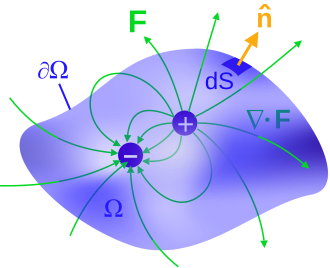
\includegraphics[width=6.5cm]{pics/div_em.png}\\
{\small Field lines (green ``spikes'') emerge from positive sources ($\div\vect{F}>0$) and terminate on negative sinks ($\div\vect{F}<0$). Draw any closed surface (the blue ``bubble'') around the region: the net flux through the bubble equals the total source strength inside it. What flows out must have been created within.}
\end{center}

\wsubsection{When to use it}

\begin{itemize}[nosep, leftmargin=*]
  \item $S$ is a complicated closed surface but $\div\vect{F}$ is simple $\implies$ compute the volume integral
  \item $S$ is not closed $\implies$ close it off with a ``cap,'' apply the theorem, then subtract the cap
\end{itemize}

\begin{example}[Divergence Theorem on the Unit Sphere]
Verify the Divergence Theorem for $\vect{F} = \vec{x,\, y,\, z}$ over the unit sphere $x^2+y^2+z^2=1$.

\wbbox{
\textbf{Volume integral side:}

1. \textbf{Divergence:} $\div\vect{F} = 1 + 1 + 1 = 3$

2. \textbf{Integrate:} $\ds\iiint_E 3\,dV = 3 \cdot \frac{4}{3}\pi(1)^3 = 4\pi$

\bigskip
\textbf{Surface integral side:}

1. \textbf{Outward normal:} On the unit sphere, $\hat{\vect{n}} = \vec{x,y,z}$

2. \textbf{Dot product:} $\vect{F}\cdot\hat{\vect{n}} = x^2+y^2+z^2 = 1$

3. \textbf{Integrate:} $\ds\oiint_S 1\,dS = 4\pi$

Both sides $= 4\pi$ \;\checkmark
}{5cm}
\end{example}

\begin{example}[Divergence Theorem on the Unit Cube]
Find the outward flux of $\vect{F} = \vec{xy,\, yz,\, xz}$ through the unit cube $[0,1]^3$.

\wbbox{
1. \textbf{Divergence:} $\div\vect{F} = y + z + x$

2. \textbf{Integrate:}
$\ds\iiint_{[0,1]^3}(x+y+z)\,dV = \int_0^1\!\int_0^1\!\int_0^1(x+y+z)\,dx\,dy\,dz$

3. \textbf{By symmetry:} $\ds\int x\,dV = \int y\,dV = \int z\,dV = \frac{1}{2}$

4. \textbf{Result:} Flux $= 3 \cdot \dfrac{1}{2} = \boxed{\dfrac{3}{2}}$
}{4cm}
\end{example}

\begin{practice}

\prob
Use the Divergence Theorem to compute $\ds\oiint_S \vec{x,y,z}\cdot d\vect{S}$ over the sphere of radius $R$.

\wans{$\wbm{4\pi R^3}$}

\vspace{2.5cm}

\prob
Use Stokes' Theorem to evaluate $\ds\oint_C \vec{-y,\, x,\, z}\cdot d\vect{r}$ where $C$ is the circle $x^2+y^2=4$, $z=3$ (CCW when viewed from above).

\wbbox{
$\curl\vect{F} = \vec{0-1,\, 0-0,\, 1-(-1)} = \vec{-1, 0, 2}$

Surface: disk $x^2+y^2\le 4$, $z=3$. Normal: $\hat{\vect{n}} = \khat$.

$\iint_S\vec{-1,0,2}\cdot\vec{0,0,1}\,dA = \iint_S 2\,dA = 2 \cdot 4\pi = \boxed{8\pi}$
}{3.5cm}

\prob
Use the Divergence Theorem to compute $\ds\oiint_S \vec{x^2, y^2, z^2}\cdot d\vect{S}$ over the unit cube $[0,1]^3$.

\wans{$\wbm{3}$}

\vspace{3cm}

\prob
Verify Stokes' Theorem for $\vect{F} = \vec{z,\, x,\, y}$ on the triangular portion of the plane $x+y+z=1$ in the first octant, with upward normal.

\wbbox{
\textbf{Surface integral side:}

$\curl\vect{F} = \vec{1,1,1}$. \; Surface: $g = 1-x-y$, so $\vec{-g_x,-g_y,1} = \vec{1,1,1}$.

$\curl\vect{F}\cdot\vec{1,1,1} = 3$. \; $\iint_D 3\,dA = 3 \cdot \frac{1}{2} = \frac{3}{2}$.

\textbf{Line integral side:} (CCW from above: $(1,0,0)\to(0,1,0)\to(0,0,1)\to(1,0,0)$)

$C_1$: $\vect{r}=\vec{1-t,t,0}$, $\vect{F}=\vec{0,1-t,t}$, $\vect{r}\,'=\vec{-1,1,0}$. Dot $= 1-t$. $\int = 1/2$.

$C_2$: $\vect{r}=\vec{0,1-t,t}$, $\vect{F}=\vec{t,0,1-t}$, $\vect{r}\,'=\vec{0,-1,1}$. Dot $= 1-t$. $\int = 1/2$.

$C_3$: $\vect{r}=\vec{t,0,1-t}$, $\vect{F}=\vec{1-t,t,0}$, $\vect{r}\,'=\vec{1,0,-1}$. Dot $= 1-t$. $\int = 1/2$.

Total: $\frac{1}{2}+\frac{1}{2}+\frac{1}{2} = \boxed{\frac{3}{2}}$ \;\checkmark
}{6cm}

\prob
Use the Divergence Theorem to derive $\text{Vol}(E) = \dfrac{1}{3}\ds\oiint_S \vec{x,y,z}\cdot d\vect{S}$.

\wbbox{
$\div\vec{x,y,z} = 1+1+1 = 3$. By the Divergence Theorem:

$\oiint_S\vec{x,y,z}\cdot d\vect{S} = \iiint_E 3\,dV = 3\,\text{Vol}(E)$

$\therefore\; \text{Vol}(E) = \frac{1}{3}\oiint_S\vec{x,y,z}\cdot d\vect{S}$. \quad $\square$
}{3cm}

\end{practice}

\end{document}
